\documentclass[11pt,twoside,abstract,notitlepage]{scrreprt}
\usepackage[utf8]{inputenc}
\usepackage{hyperref}
\hypersetup{
	colorlinks=true,
	linkcolor=black,
	citecolor=black,
	filecolor=black,
	urlcolor=blue
}
\usepackage{verbatim} 
\usepackage{setspace}
\usepackage{graphicx}
\usepackage{caption}
\usepackage{color}
\usepackage{index}
\usepackage{listings}
\usepackage{tabularx}

%\onehalfspacing
\setstretch{1.0}
\newindex{todo}{todo}{tnd}{Todo List} 
\newcommand{\todo}[1]{
    %\textcolor{red}{[To do: #1]}\index[todo]{#1} 
}
\hyphenation{}

\lstset{numbers=left, showspaces=false, showstringspaces=false, showtabs=false, tabsize=2, language=[ANSI]C}

\begin{document}


\pagenumbering{none}
\title{Development of a protocol stack for an embedded operating system\break
Entwicklung eines Netzwerkstacks für ein eingebettetes Betriebssystem}
\author{Erasmus Schröder, Berlin Institute of Technology\\
    Communication and Operating Systems\\
    rasco@cs.tu-berlin.de}
\maketitle



\vfill
\vfill
\vfill
\begin{center}\begin{minipage}{0.89\textwidth}

Die selbstständige und eigenhändige Ausfertigung versichert an Eides
statt:

\bigskip{}
\bigskip{}
\bigskip{}
Berlin, den \today \\ \vspace{2cm} \hfill \parbox{6cm}{\centering \rule{6cm}{1pt} \\ Erasmus Schröder}
\end{minipage}\end{center}\vspace*{-5cm}
\newpage
\begin{abstract}
We describe the development of a minimal communications stack for an embedded operating system. It consists of modules which, together, form an interface through which user applications can communicate over UDP/IP and TCP/IP. An ethernet interface for AT91RM9200 microcontrollers is provided, but other link layer interfaces can be created. The modularity of the implementation should allow integration into both monolithic and microkernel operating systems.
\end{abstract}

\renewcommand{\abstractname}{Zusammenfassung}

\begin{abstract}
Im folgenden wird die Entwicklung eines minimalen Netzwerkstacks für ein eingebettetes Betriebssystem beschrieben. Der Stack besteht aus Modulen, die zusammen eine Schnittstelle ergeben, die Anwendungsprogrammen ermöglicht, per UDP/IP und TCP/IP zu kommunizieren. Eine Ethernet-Schnittstelle für AT91RM9200 Mikrocontroller ist vorgegeben, aber die Einbindung anderer Verbindungsschichtmodule ist möglich. Die Modularität dieser Implementation sollte Integration in monolithische- sowie Mikrokernelbasierte Betriebssysteme erlauben.\end{abstract}
\newpage
\setcounter{tocdepth}{3}
\tableofcontents



\newpage

\pagestyle{headings}
\pagenumbering{arabic}
\chapter{Introduction}
The Communication and Operating Systems (KBS) research group of the Berlin Institute of Technology is, amongst other things, conducting research on Distributed Swarm Operating Systems and teaching students in operating system design. For these purposes, ARM9TDMI-based taskit Portux 920T Mini-PC microcontrollers are employed \cite{taskit}. 

A research objective is to design and develop a distributed mobile operating system. FlockOS (federation of linked objects with common tasks operating system) should provide transparent communication and synchronization to applications and abstract from single devices \cite{flockos}.

\section{Problem statement}
Of course such a system needs networking capabilities to communicate with peers or other nodes locally, or over the internet. The AT91RM9200's peripherals include an Ethernet MAC (Media Access Control), which can be used to create links between machines and send or receive data. But this (Link Layer) interface on its own does not provide everything that is needed in a proper internetworking application. Requirements for complex networking applications include transmission reliability, port multiplexing and routing. Furthermore, communication with heterogenous hosts, such as ones that don't have an ethernet interface, should be possible.  

The platform should be able to communicate over common protocols, such as the Internet Protocol (IP) and Transmission Control Protocol (TCP) which would enable communication with ordinary desktop computers or remote peers in other networks over the internet.

The protocol stack should be modularly designed and have clearly defined interfaces to allow integration into both monolithic and microkernel operating systems. 

\section{Organisation of the Thesis}
Section II. offers the technical background knowledge that is necessary to reach this goal. The Berkeley Sockets API, popular TCP/IP implementation is presented. 
A bottom-up approach is taken to explain the Internet Protocol Suite and its various layers, beginning with the physical layer (Ethernet) followed by the network layer (IP) up to the transport layer (UDP, TCP). Hardware details of the Portux920T Mini-PC are illustrated and a some standards and protocols (including TCP/IP) related to internetworking are explained.

In section III., Approach, the architecture of the stack is illustrated and justified. Requirements for the carrying operating system are defined. Standard compliance and limitations are discussed.

The Implementation section describes the interior architecture of the resulting protocol stacks by following the path that a packet takes through the different layers. The resulting application programming interface is defined and explained. The interfaces are described in detail in order to facilitate porting.

In section V., the resulting software is evaluated and compared to other existing systems. Throughput and latency tests in different scenarios are performed and discussed. Limitations and restrictions are discussed.

In the final conclusion its usefulness, compatibility, reusability and extensibility are examined and prospective options are debated.

\chapter{Technical Background}
For almost thirty years IP has been the global standard in computer networking. Although the Internet Protocol has hardly changed over this time, it is still by far the most widely used | if not the | way to communicate across networks. The combination of TCP/IP is used for e-mail transmissions, viewing web pages, transferring files and many other network services. Since IPv4, the original Internet Protocol, IPv6, a new version, has emerged, but has not yet taken over the majority of links. This is mostly due to the trouble associated with changing the structure of a complex network without sacrificing uptimes and reliability.

This chapter provides background information about the inner working of the internet. The embedded hardware, the taskit Portux920T used in this task, is described and a programmer's viewpoint to sockets is outlined. 

\section{Networking overview}
From a user's point of view, the communications stack is an abstract channel that takes and outputs data from our program to the receiver and receives and inputs data into our program from the sender. What kind of physical medium we are trasmitting on, which route is taken to reach the destination or how fast we can write data is not of concern to the user. These, and other things, are performed by the protocol stack. 

The Internet Protocol Suite describes the protocols, including TCP/IP, as used in today's internet. It started as a research and development program initiated by the Defense Advanced Research Projects Agency (DARPA) by the U.S. Department of Defense but later gained popularity in civilian fields. Today, the IP suite and its standards are controlled by the Internet Society (ISOC), a non-profit organization, and its various suborganizations, the Internet Engineering Task Force (IETF), the Internet Architecture Board (IAB) and the Internet Research Task Force (IRTF) \cite{isoc}. 



\paragraph{Layers} The Internet Protocol Suite defines a set of layers, each layer handling different communication aspects. Each of the protocols involved resides in one of the four layers. The layers are pictured in figure \ref{fig:iplayers}. 


On top is the user program (\emph{Application Layer}), while on the bottom lies the physical link (\emph{Link Layer}). The user data (e.g. Hyper Text Transfer Protocol for viewing web pages) is encapsulated in a \emph{Transport Layer} protocol (e.g. TCP). This protocol is then encapsulated in an IP packet (\emph{Internet Layer}) which in turn is encapsulated in a \emph{Link Layer} frame. The network interface device then sends the data. When it arrives at its final destination the receiving stack reverses the encapsulation and passes the data to the receiving user program.  Figure \ref{fig:iplayers} illustrates the path that is taken through the layers. Each layer performs a different set of tasks required for data exchange between two endpoints.

\begin{figure}

\centerline{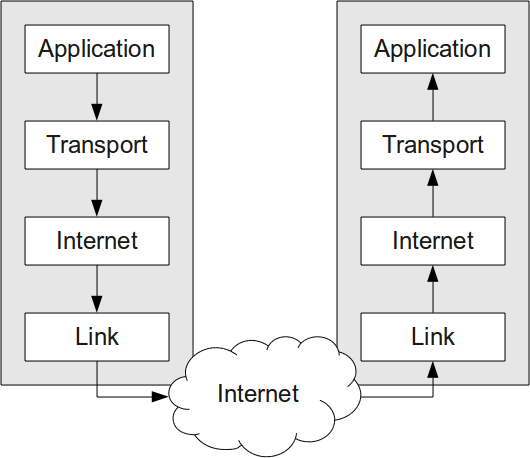
\includegraphics[width=0.5\textwidth]{images/iplayers.png}}
\caption{The layers involved when two applications communicate (note: the 'Internet' cloud in this picture hides possible routing points)}
\label{fig:iplayers}
\end{figure}

\begin{itemize}
	\item Ethernet network interface cards or other network interfaces, such as IEEE 802.11 (wireless local area networks) belong to the \emph{Link Layer} and are responsible for the physical transmission of bits from one point to another. Their purposes include detecting collisions on shared media since many participants can use the same shared cable or frequency at the same time (imagine a group of people talking at the same time).

    \item The \emph{Internet Layer} is in charge of moving packets across networks using the underlying physical link. This way, even although two endpoints might use different Link Layer protocols, the IP is their common denominator. Packet routing also happens on this layer. 

    \item The \emph{Transport Layer} protocols further abstract from endpoints. They provide port numbers which are used to identify which process on a machine is communicating with which process on another machine (multiplexing).
    
     The Transmission Control Protocol, amongst other services, also provides reliability (in case of packet loss or delayed arrival). In computer networks, data that was sent is not guaranteed to arrive. Also, in packet-switched networks with multiple routers such as the internet, packets can be delayed and arrive out of order. TCP achieves reliability by sending acknowledgements for received packets and resending packets for which no acknowledgement was received after a certain timeout. 
     
    \item Finally, in the \emph{Application Layer} reside the programs that initiate the communication. Widely know Application Layer protocols include HTTP for web browsing, SMTP for sending e-mail or FTP for transferring files. They all use TCP as their transport protocol.
\end{itemize}

All of the Internet Protocol Suite's official standards are available as RFC (Request For Comment) documents on the IETF's web page \cite{ietf}. The RFCs are text documents that have unique serial numbers, higher numbers being newer publications. RFC 1122, \emph{Requirements for Internet Hosts -- Communication Layers}, is one of the key RFC's of the Internet Protocol Suite. RFC 791 and 793 go into more detail and describe the IP and the TCP, respectively. They are used for implementation and describe the workings of the protocols. We will use RFCs extensively throughout the implementation process \cite{stevens94}.


\section{The Portux 920T} 
The taskit Portux 920T Mini-PC is an embedded PC with an AT91RM9200 system-on-chip. The AT91RM9200 consists of a 32-bit ARM9TDMI-based ARM920T processor core and 16K bytes of on-chip SRAM and 128K bytes of ROM \cite{atmel}. Peripherals include USB Host and Device ports, a 10/100 Base T Ethernet MAC and two serial interfaces. It has an advanced interrupt controller (AIC), a real time clock (RTC) and a memory management unit (MMU). The processor runs at 200 MIPS (million instructions per second) at 180 MHz. The board comes with 64 MB of SDRAM and 16 MB Flash memory. This hardware allows for the running of modern operating systems. The board comes with a preinstalled Linux distribution and U-Boot bootloader. 

\begin{figure}
\normalsize
\centerline{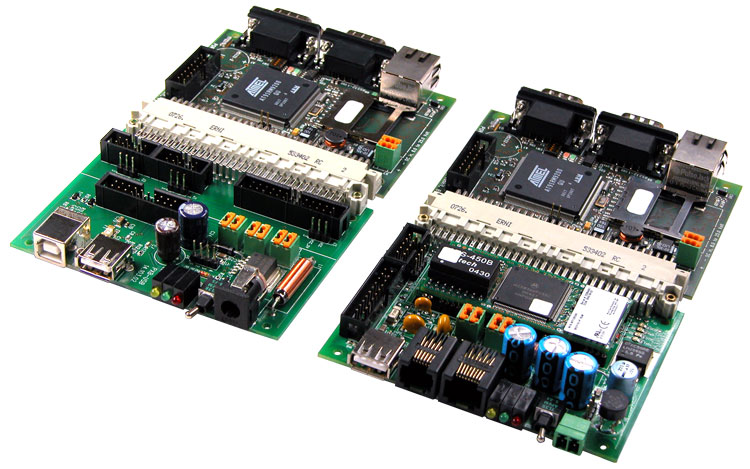
\includegraphics[width=0.8\textwidth]{images/portuxminipc.jpg}
\label{fig:portuxpicture}}
\caption{taskit Portux920T}
\end{figure}

\paragraph{EMAC} The EMAC (Ethernet Media Access Control) acts as the interface between the physical transceiver and the logical link layer. It lets us transmit logical blocks of data (so-called Ethernet frames) over a physical medium, without having to worry much about the physical aspects of data transmission (digital modulation, synchronization, collision detection and so on). The EMAC is connected to the Advanced Interrupt Controller. Interrupts can be generated on receive and transmit completion and other events. The AIC and the EMAC have to be configured appropriately for interrupt-generation to work.

The link layer protocol is situated at this level. All IP packets that are to be transmitted are encapsulated in an Ethernet frame. In our implementation Ethernet II frames are used. Each communicating party has a unique 6-byte hardware address that identifies it. The frame contains the destination hardware address at the beginning, followed by the source hardware address, and a type field. The type field is used to determine which upper layer protocol (e.g. IP or ARP) is contained in the frame. The last four bytes of every Ethernet frame contain a checksum to verify the validity of the received data. If the frame is of type IP, it is passed on to the IP stack; if it is an ARP (Address Resolution Protocol) frame, it is passed on to the ARP code, and so on (ARP is described in the next section) \cite[p. 98]{stevens95}.

\section{The Internet Protocol} 
The Internet Protocol as described by DARPA in RFC 791 \cite{rfc791} is a protocol that provides transmitting blocks of data between specified source and destination machines in packet-switched networks. The block size can be adjusted and IP datagrams can be fragmented to fit into networks that (perhaps because due to limitations of their physical medium) support only smaller packet sizes.

IP has no reliability or multiplexing mechanisms but rather, in practice, acts as a capsule to transmit other protocols that do have these mechanisms. The IP stack passes forward its outgoing data to the link layer, which takes care of physical transmission to a destination (not necessarily the destination specified by the IP, but to the next gateway). 

\paragraph{IP addressing}
IP is a network layer (internet layer) protocol, and it is here that the global addressing on the internet occurs. Every IPv4 packet contains the 32-bit source and destination addresses (commonly called IP addresses) that specify where the packet comes from and where it should be sent. 

The way an IP packet reaches its destination on the internet happens through routing. The internet is effectively a network of networks interconnected by routers that forward packets to the appropriate destination. Internet Service Providers (ISPs) are the networks, and they do the routing on the internet. A router is a communication device that operates on the IP layer and contains a table of routing destinations. The routing table tells it where to forward a packet depending on its destination address. 

ISPs have a certain range of addresses that they can give to their customers. The ISPs are assigned their address range by the Internet Assigned Numbers Authority (IANA) which acts as a global manager of IP address spaces.

\begin{figure}
\small
\renewcommand{\arraystretch}{1.2}
\caption{The IPv4 packet header}
\label{ipheader}
\centering
\begin{tabularx}{\textwidth}{|X|X|X|X|X|}
\hline
0-3 & 4-7 & 8-15 & 16-18 & 19-31 \\ \hline
version & header length & type of service & \multicolumn{2}{c|}{total length} \\ \hline
\multicolumn{3}{|c|}{identification} & flags & fragment offset \\ \hline
\multicolumn{2}{|c|}{time to live} & protocol & \multicolumn{2}{c|}{header checksum} \\ \hline
\multicolumn{5}{|c|}{source address} \\ \hline
\multicolumn{5}{|c|}{destination address} \\ \hline
\multicolumn{5}{|c|}{options} \\ \hline
\end{tabularx}
\end{figure}

\begin{figure}
\normalsize
\caption{Example: the path an e-mail takes through the internet goes through several routers and ISP networks before arriving at its final destination}
\centerline{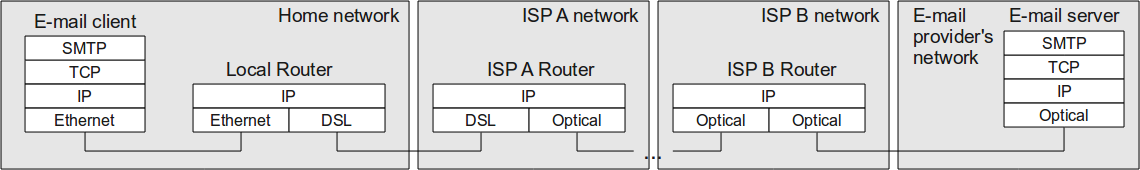
\includegraphics[width=1.0\textwidth]{images/routing.png}
\label{fig:routing}}
\end{figure}

Of course not only ISPs pose networks. Through subnetting subnetworks can be created. One ISP can even be a subnetwork of another, bigger ISP, or a large enterprise can have its own subnetwork. Subnetting allows nodes to determine which network they are in and whether a given IP address is located in another network. 

Figure \ref{fig:routing} shows an example of routing and subnetting. To send e-mail an SMTP client on a computer in a home network sends IP packets containing the e-mail content to a remote SMTP (Simple Mail Transfer Protocol) server. The client machine's protocol stack examines the destination IP address and determines that the receiver is not on the same subnet. The packet is therefore sent to the local gateway, which in turn forwards the packet through an active DSL connection to the client's ISP (ISP A). ISP A takes care of routing the packet to the ISP that the mailserver is connected to (ISP B). This can involve many intermediate routers and ISPs from different geographical locations. Finally, ISP B passes the packet to the e-mail server which can read the packet's source address and respond appropriately.

\todo{more IP details?}


\paragraph{Address Resolution Protocol} We have now seen two types of addresses: the 6-byte hardware address in the Ethernet frame and the 4-byte IP address. But how does a computer connected to an ethernet know which hardware address to specify when it wishes to send an IP packet? 

ARP, the Address Resolution Protocol, is a protocol used to determine another host's hardware address. When an IP packet shall be sent, the protocol stack relies on an ARP table to lookup the hardware address for the specified IP. If the table does not contain an entry for that address, an ARP request is broadcast (using the special broadcast address) and the packet is delayed. When an ARP request addressed to the local IP address is received, an ARP reply including the local hardware address is sent back to the sender. The receipt of an ARP reply triggers the sending of delayed packets for that destination and updates the ARP table.

In the example from figure \ref{fig:routing}, the client would send an ARP request for the local router's MAC address and wait for the reply before sending any SMTP data. 




\section{User Datagram Protocol} 
UDP is a very simple datagram-oriented transport protocol. It does not abstract from the fact that data is transmitted in packets. This means that each send call by a program causes exactly one UDP packet and one IP packet to be sent. UDP is connectionless and the process needs to keep track of its connections itself. Each time a datagram is to be sent, the process must specify the destination address and whenever a datagram is received, the process is given the address of the sender.

The UDP header consists of 16-bit source and destination port numbers. It contains a 16-bit length field that holds the length of the data including the UDP header and an optional 16-bit checksum for the header and the data. 

\begin{figure}
\renewcommand{\arraystretch}{1.2}
\caption{The UDP header}
\label{udpheader}
\centering
\begin{tabularx}{\textwidth}{|X|X|}
\hline
0-15 & 16-31 \\ \hline
source port & destination port \\ \hline
length & checksum \\ \hline
\end{tabularx}
\end{figure}  

Because of its simplicity compared to stream-oriented, reliable protocols, UDP performs faster than TCP. It is therefore often used in applications where packet loss can be tolerated up to a certain level and throughput and latency requirements are high. Such applications include video streaming, internet telephony or real-time games.

\section{Transmission Control Protocol} 
The Transmission Control Protocol, unlike UDP, provides a connection-oriented service between two applications. The protocol keeps track of the connection state  and so is able to offer a reliable ordered byte-stream. 

TCP is the most complex and most popular transport protocol in the IP suite. RFC 793 \cite{rfc793} specifies the Transmission Control Protocol and RFC 1122 \cite{rfc1122} adds some important features to its original specification, such as congestion control. 

Since packets can arrive out of order, be corrupted or never arrive, a protocol taking care of reliable transmission was needed. TCP achieves this through the use of sequence numbers and acknowledgements. Every TCP segment sent contains a sequence number and an acknowledgement number and the connection keeps maintains the state of these numbers. Figure \ref{tcpheader} depicts the TCP header. Just like UDP, TCP multiplexes packets by using source and destination port numbers. 

 Every data packet sent must be acknowledged by the receiver. The acknowledgement occurs through the sending of a TCP packet with the acknowledgement number set to the sequence number of the acknowledged packet plus its length. So, for example, a packet with the sequence number 5 of length 20 would be acknowledged by sending a packet with an acknowledgement number of 25.

This way the sender knows how many bytes the receiver has acknowledged. The 32-bit long unsigned sequence numbers are compared in two's complements so that wrapping does not corrupt the comparison, because the sequence number one 1 is greater than the sequence number $2^{32}-1$.
 
After a certain timeout the sender retransmits the packet. This occurs transparently to the application layer protocol which does not need to interfere with retransmissions. The packets are queued in a retransmission buffer until they have been acknowledged by the other side.

On the receiver side a receive buffer takes incoming packets and examines their sequence number. If the sequence number matches the next expected sequence number, the data can be passed on to the user application and an acknowledgement can be sent. 

An out of order buffer which stores packets with sequence numbers that are higher than expected can also be implemented. As soon as a packet, which fills a gap between an out of order packet and the next expected sequence number, arrives, the out of order packet can be acknowledged and passed to the application. Out of order buffering greatly enhances the performance when a single packet is lost. The reason for this lies in the fact that the sending TCP can resend the packet because it can assume that it has been lost on the way since the receiver never acknowledged it.

\paragraph{Connection establishment}
A connection is established by a three-way handshake and can be made simultaneously by both parties. The initial state of a TCP socket is the closed state. An active connection opening by the application results in a synchronization segment being sent and the socket state is put in the SYN\_SENT state. A passive connection opening waits for a synchronization segment to arrive. Once a synchronization segment has been acknowledged, the connection is established. Figure \ref{fig:tcpstatediagram} shows a simplified state transition diagram of the TCP. 

\paragraph{Connection termination}
A connection can be terminated by sending a FIN segment. The receiving application is informed by the TCP stack that the remote host wishes to terminate the connection. Connection termination is also acknowledged by both sides. 

\paragraph{Flow control}
In the case of a slow receiver and a fast sender, TCP employs a method of flow control. This is achieved by the advertisement of a so-called receive window in every segment. This receive window tells the sender how many bytes the receiver's buffer can hold, so it can adjust its rate of sending accordingly. 

\paragraph{Congestion control}
Congestion control prevents the congestion of the network. It is detected by the sending party when duplicate acknowledgements arrive. The congestion control algorithm is used in combination with a slow-start algorithm. Slow start means that the sender will begin sending slowly but will increase its rate additively. The slow start algorithm is aborted when packet loss is detected and the sender switches into congestion control mode. 


%\begin{comment}
\begin{figure}
\small
\renewcommand{\arraystretch}{1.2}
\caption{The TCP header}
\label{tcpheader}
\centering
\begin{tabularx}{\textwidth}{|X|X|X|X|}
\hline
\multicolumn{3}{|c|}{0-15} & 16-31 \\ \hline
\multicolumn{3}{|c|}{source port} & destination port \\ \hline
\multicolumn{4}{|c|}{sequence number} \\ \hline
\multicolumn{4}{|c|}{acknowledgement number} \\ \hline
header length & reserved & control flags & window size \\ \hline
\multicolumn{3}{|c|}{checksum} & urgent offset \\ \hline
\multicolumn{4}{|c|}{options} \\ \hline
\end{tabularx}
\end{figure}
%\end{comment}

%\begin{comment}
\begin{figure*}
\normalsize
\centerline{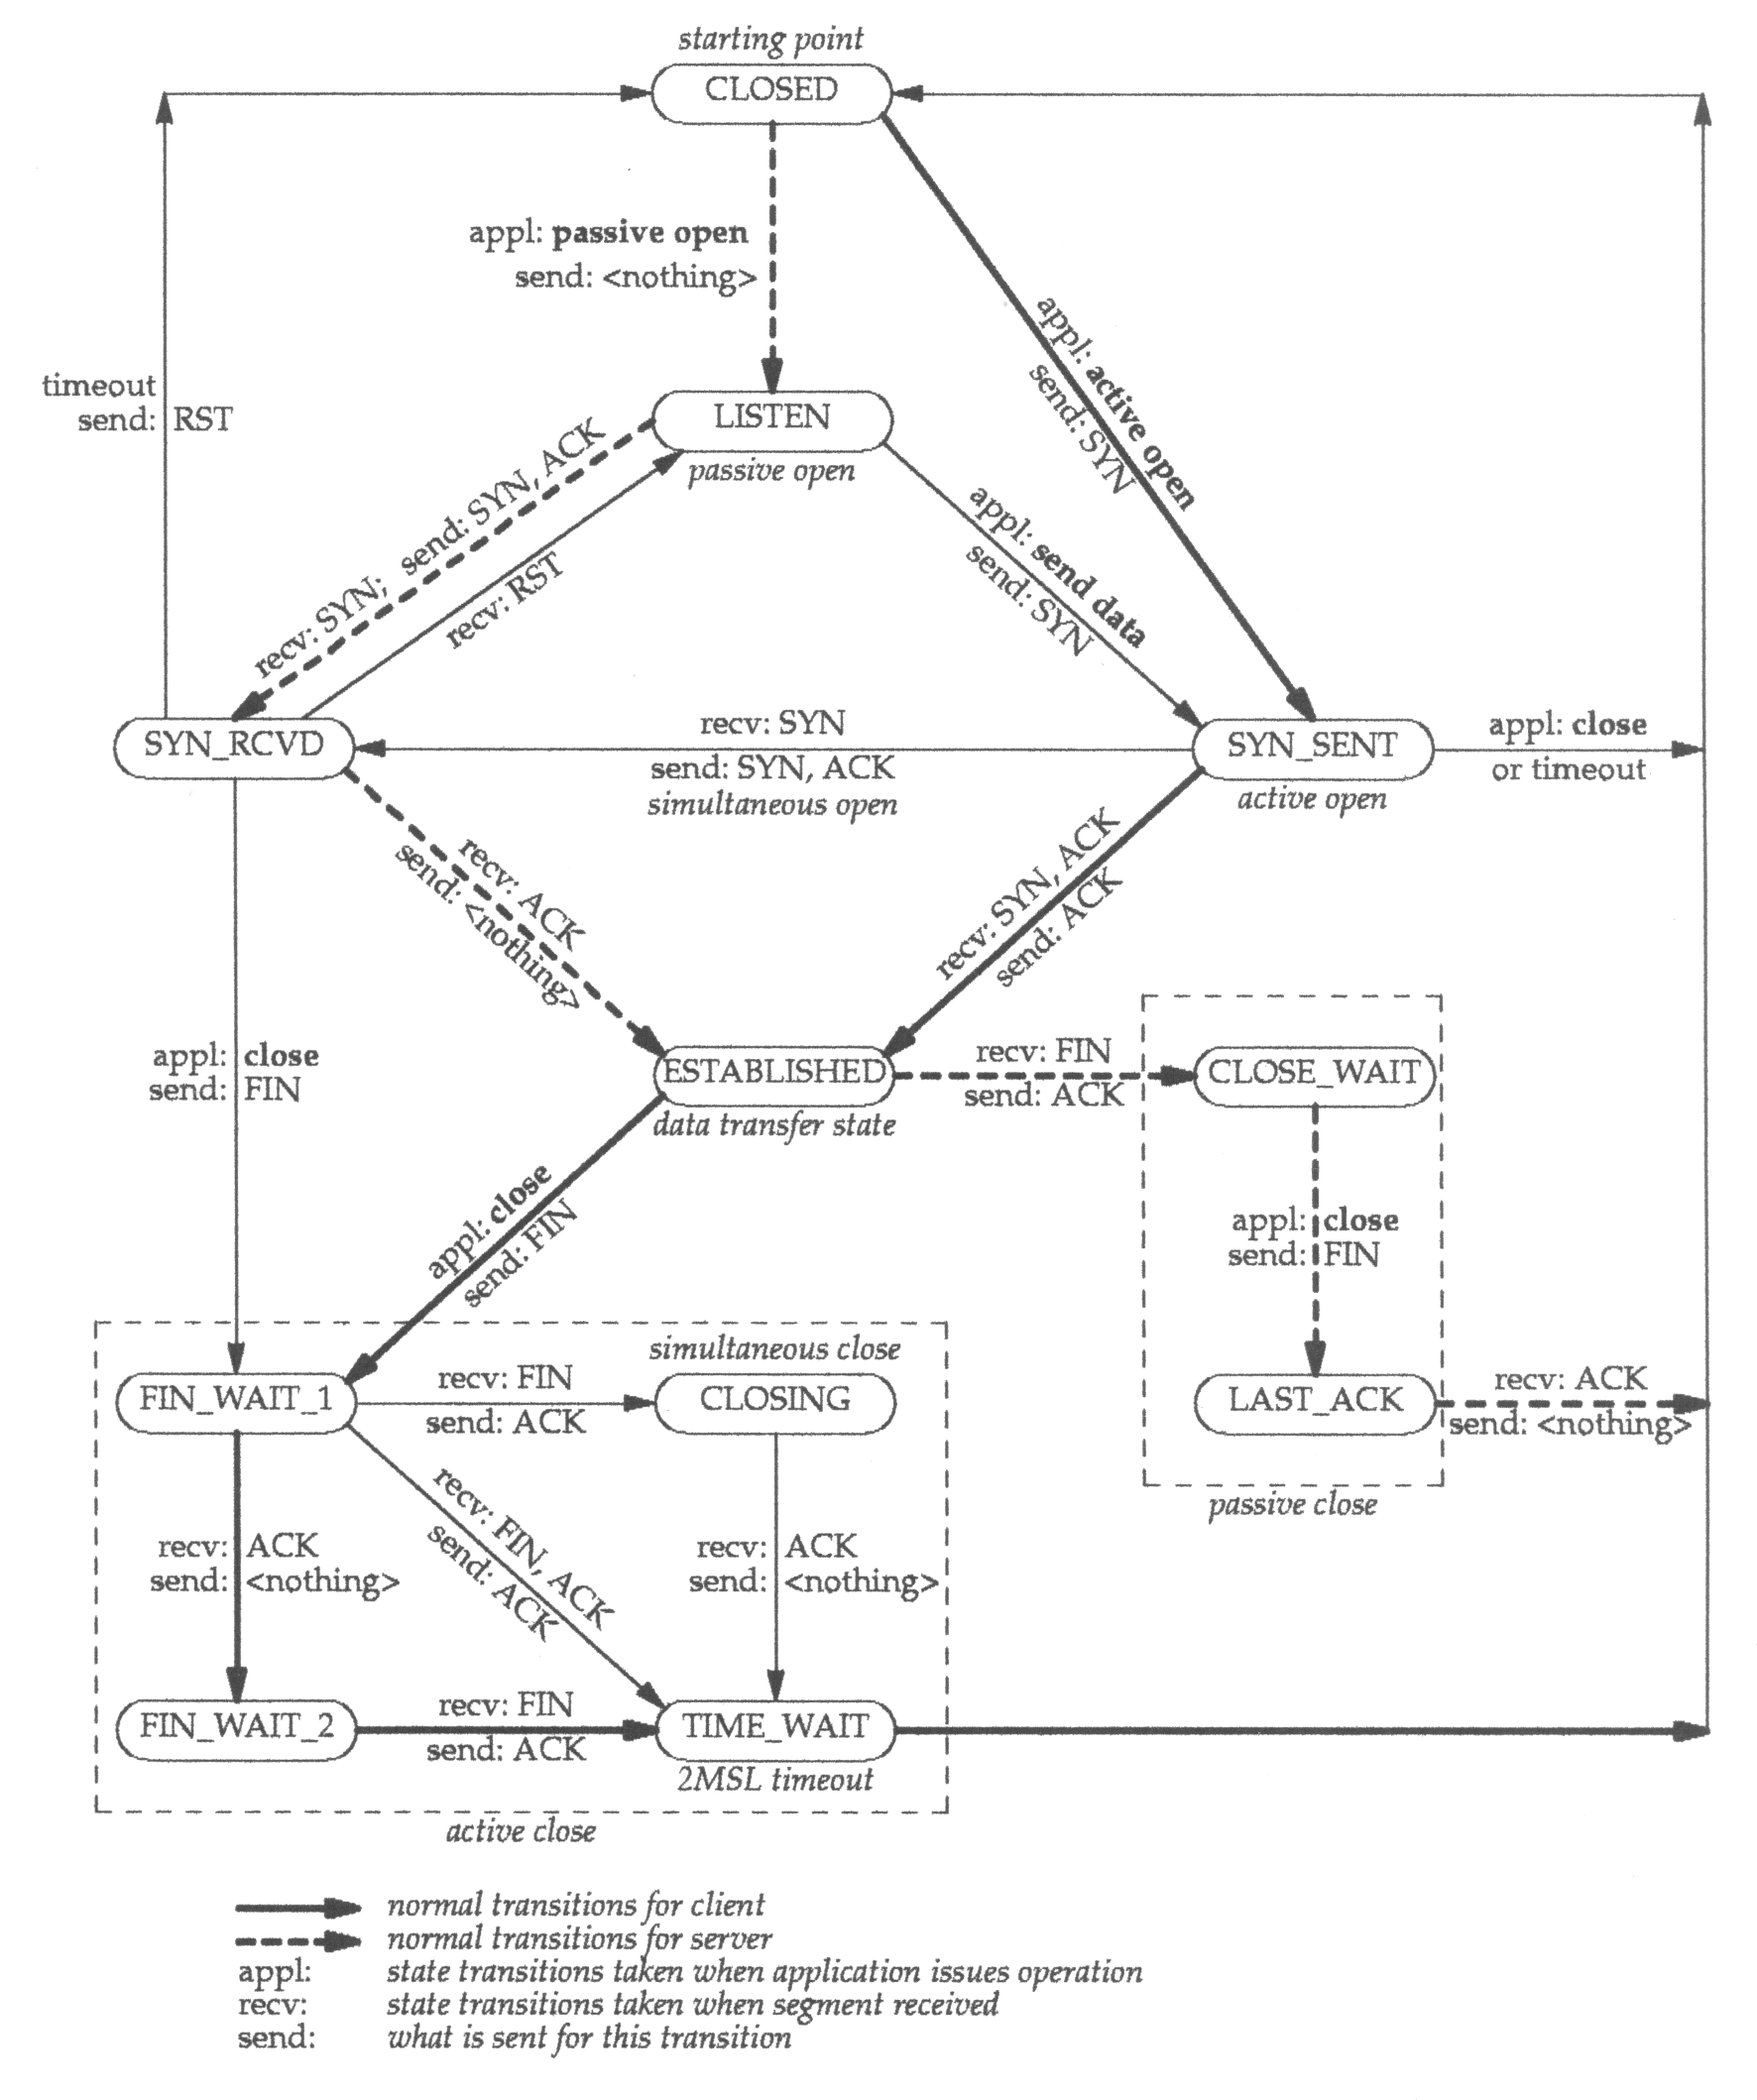
\includegraphics[width=1.0\textwidth]{images/state-diagram-big.png}
\label{fig:tcpstatediagram}}
\caption{TCP state transition diagram}
\end{figure*}
%\end{comment}


\section{Socket programming and Berkeley sockets} 
The way a programmer interacts with network communication usually takes place through network sockets. Sockets are an abstraction from the lower-level communication going ahead. They are the programming interface to the protocol stack.

As can be seen by looking at BSD socket functions, the socket programming interface hides the lower protocol layers from the user. The programmer only needs to know about his or her own application layer protocol. Conversely, the lower layer protocols need to know nothing about what is going on at the application level.

In most applications the client-server model is used. This means that one side acts as the server that listens for incoming connections and the other side acts as a client who initiates the connection. For example, when we visit a web page, we act as the client, and our request is answered by a webserver. Most servers are active around the clock and are designed to serve multiple clients in parallel. Some applications don't use the client-server model, but rely on peer-to-peer communication instead. In this model, each communication participant is, in a way, both a server and a client.

\paragraph{BSD sockets} The Berkeley sockets API (Application Programming Interface) is the de facto standard abstraction of network sockets. It originated from the BSD Unix (Berkeley Software Distribution) operating system, a UNIX derivative. Because of the open source nature of its release, this API has been ported to many other systems. Most of the popular operating systems' socket interfaces are compatible, or widely compatible, to the BSD sockets API. 

Figure \ref{fig:berkeleysockets} lists the most noteworthy of functions a process can use to interact with sockets \cite[p. 445]{stevens95}. This listing is simplified and does not include configuration parameters. 

\begin{figure}
\caption{Some functions of the Berkeley sockets API}
\label{fig:berkeleysockets}
\renewcommand{\arraystretch}{1.2}
\begin{tabularx}{\textwidth}{l|X}
\textbf{function name} & \textbf{description} \\ \hline
socket & creates a new socket using the specified protocol (e.g. TCP/IP) \\ \hline
bind & binds the local address of the socket to the one specified \\ \hline
connect & establishes a connection to the specified host  \\ \hline
close & terminates the current connection of the specified socket \\ \hline
send & sends data on the specified socket \\ \hline
recv & receives data from the specified socket \\ \hline
sendto & sends data on the specified socket to the specified host \\ \hline
recvfrom & receives data from the specified socket and returns the sender's address \\ \hline
listen & makes the socket passive, meaning that it will listen for incoming connection requests, rather than actively connecting (used for servers)\\ \hline
accept & accepts an incoming connection request after the \emph{listen} call\\ \hline
select & waits for a socket from a set of sockets to finish reading or writing\\ 
\end{tabularx}
\end{figure}

A process that wants to communicate over the internet starts with the creation of a socket by calling the \texttt{socket} function. It specifies which protocol it wants to communicate over (e.g. TCP/IP or UDP/IP). This call triggers the the protocol stack to reserve space for the socket the identifier of the newly-created socket returns. The identifier is used in subsequent calls to the other functions to indicate which socket they should operate on.

By calling \texttt{bind}, a socket's local address is set to the address specified by the caller. This is mostly of interest for servers that wish to listen on a specific port. Most application protocols have well-known ports, so that clients know what port to connect to when they want to access a specific service.

For connectionless transport protocols like UDP, the process can start sending and receiving data immediately through the use of the \texttt{sendto} and \texttt{recvfrom} functions. For connection-oriented protocols like TCP, \texttt{send} and \texttt{recv} are used, but the socket will have to be connected first (using the \texttt{connect} call). A connected socket receives only data from the host it is connected to.

\texttt{connect} initiates a connection with the specified host. For TCP this means a three-way handshake with the remote partner. The calling process is blocked until the connection has either been successfully established or an error has occurred. All subsequent send and receive operations will use the remote host for their address. A UDP socket can also be connected to achieve this, although no handshake or exchange whatsoever is made.

\texttt{close} has two uses: On the one hand it is used to close the connection to the remote host and on the other hand it is used to delete the socket. \texttt{close} must be called on every socket (created using \texttt{socket}), once communication is done.

\texttt{listen} (for connection-oriented protocols) is used by servers (and sometimes passive clients) to wait for incoming connection requests (initiated by the call to the \texttt{connect} function). The function blocks the process and returns when a connection request is received on the socket. Incoming connection requests are accepted by a call to \texttt{accept}. \texttt{accept} returns the identifier of a new socket which is in connected state. This new socket is from then on used to interact with the client, while the original listening socket stays in its listening state, ready to accept new connections. 

The \texttt{select} call is especially useful for server applications because it can multiplex several socket events into one function call. \texttt{select} blocks the process until an event (e.g. a read) on one out of the specified set of sockets occurs. 

In addition to blocking the process, all socket functions can be configured to be non-blocking or to return after a specified timeout. 



\chapter{Approach}
This chapter provides an overview of the the protocol stack's structure and modular composition and defines system requirements for running the stack. 

FlockOS, the actual motivation for the stack, was still in early concept stage when this document was written, so a very basic operating system was built specifically for the purpose of testing the stack. An advantage of the simplicity of the system was that it was straightforward to extend. Another advantage was that requirements were easily defined.

\section{Requirements}

The testing operating system is a basic round-robin multitasking kernel. Multitasking is an important requirement because we want the final stack to be able to multiplex information in a microkernel environment and to provide its service to multiple processes concurrently (as pictured in figure \ref{fig:multiplexing}). Furthermore, a system call environment has to be provided, or (for microkernel systems) interprocess communication, so that the processes can call the API functions. The kernel has to provide a way to pause a process that is waiting for a particular resource. A basic timing mechanism is needed for TCP timeouts. 

\begin{figure}
\caption{Different processes using the same stack for communication}
\vspace{0.3cm}
\label{fig:multiplexing}
\centerline{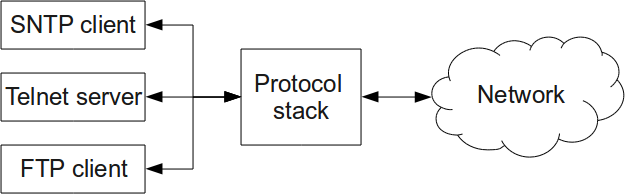
\includegraphics[width=0.6\textwidth]{images/multiplexing.png}}
\end{figure}

The protocol stack relies on a kernel memory module to allocate memory dynamically for its internal buffers. 

No 'proper' memory management and memory protection was present in the testing environment, which means that those stack functions that interact with user data do therefore not check for locality. Extending the stack to support this on a system with memory protection should not be too troublesome, since the parts that have to be modified for this lie exclusively in user API functions. 

Also resulting from the lack of memory management the data buffers used by the protocol stack reside in kernel memory and not in user memory, but their size can be configured. Changing the stack to store user structures in user memory would require replacing their respective kernel memory allocation calls for buffers with user allocation calls. These calls reside almost exclusively in the input and output functions.

The kernel also needs to handle the Ethernet MAC's IRQ (Interrupt Request) in order to be able to receive packets. This (besides the System Timer) is the only IRQ that is really necessary. 

TCP needs a random number generator which is not provided by the hardware, so a pseudo random-number generator has to be supplied. A way to do this is the use of timestamps as seed numbers. This method is further discussed in the implementation section.

\section{Architecture}
The protocol stack consists of five modules: \textbf{ethernet}, \textbf{arp}, \textbf{ip}, \textbf{udp} and \textbf{tcp}. All function calls and variables of a module are prefixed with the module's name and an underscore (such as \texttt{tcp\_input} or \texttt{ethernet\_irq}). This helps reading and maintaining the code and prevents ambiguity errors when the boundary between two modules is not clear. Figures \ref{fig:output} and \ref{fig:input} illustrate the relation of the modules to each other. 


\paragraph{Output} When an output operation is issued by a process, udp\_output or \texttt{tcp\_output} is called, depending on the type of the socket (see figure \ref{fig:output}). After processing, these functions pass the data over to the \texttt{ip\_output} function which prepends an IP header containing the destination IP address. This IP datagram is handed over to the ethernet module for sending. But before the ethernet module can send the frame it needs to know the destination hardware address. A call to \texttt{arp\_resolve} of the ARP module looks up the MAC address for the IP from the ARP table. If no entry for the IP address is found, \texttt{arp\_send}, which sends and ARP request, is called and the packet is buffered for later sending.
\begin{figure}
\caption{Relation of the modules on an output event}
\vspace{0.3cm}
\label{fig:output}
\normalsize
\centerline{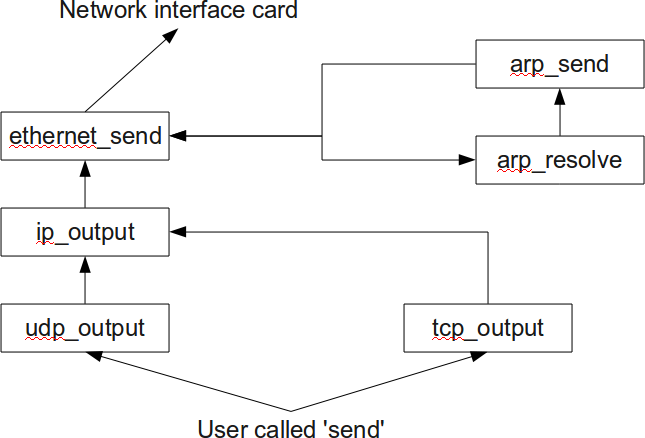
\includegraphics[width=0.5\textwidth]{images/output.png}}
\end{figure}



\paragraph{Input} An input event is triggered by the operating system's interrupt request handler (see figure \ref{fig:input}). The ethernet IRQ handler is called by the kernel and checks whether a frame has arrived. If this is the case, it distinguishes between ARP and IP and passes the frame forward accordingly. In the case of an IP packet, the \texttt{ip\_input} function is called. \texttt{ip\_input} then calls the input function of the UDP or the TCP module, depending what kind of packet arrived. The transport protocol passes the data over to the receiving socket (or discards it if no matching socket is found). If the received frame contained an ARP reply, all packets buffered for that destination are sent.

\begin{figure}
\caption{Relation of the modules on an input event}
\vspace{0.3cm}
\label{fig:input}
\normalsize
\centerline{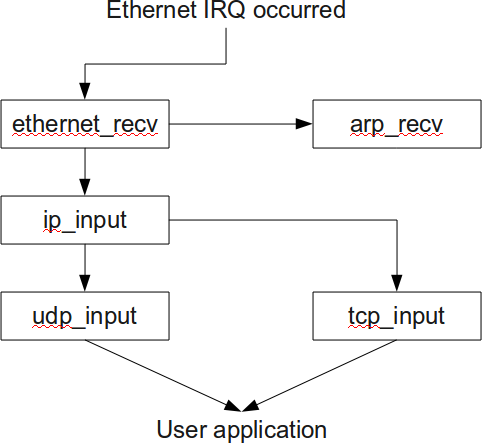
\includegraphics[width=0.4\textwidth]{images/input.png}}
\end{figure}

\paragraph{Timing} The TCP module uses a global timer for retransmission timeouts, connection establishment timeouts and connection termination timeouts. The ARP module needs timeouts for cache invalidation and updating.

\section{Standard compliance}
RFC 791 \cite{rfc791}(Internet Protocol), RFC 768 \cite{rfc768} (User Datagram Protocol) and RFC 793 \cite{rfc793} (Transmission Control Protocol) act as guidelines for implementation. An implementation not following the standards may not be able to communicate correctly with other protocol stacks. 

RFC 1122  corrects the aforementioned RFCs and adds details and improvements. In section 4.2.5 | "\texttt{TCP REQUIREMENT SUMMARY}" a list of TCP features is given \cite[p. 108]{rfc1122}. The table specifies which features an implementation can, should, or must realize, and what behavior an implementation should not or must not have.  

Some features that can be left out without rendering the stack completely useless include round-trip time estimation, certain TCP and IP options, congestion control, flow control, multiplexing in a multitasking environment and queuing out of order segments. Figure \ref{fig:features} shows which features the current implementation serves. 


\begin{figure}
\caption{A list showing which features were implemented}
\label{fig:features}
\renewcommand{\arraystretch}{1.2}
\begin{tabularx}{\textwidth}{X|X|X}
Feature & Implemented? Required? \\ \hline
TCP flow control & yes & yes\\ \hline
TCP timers & yes & yes \\ \hline
TCP Retransmissions & yes & yes \\ \hline
TCP out of order data reordering & partial & no \\ \hline
TCP urgent data & no & yes \\ \hline
TCP congestion control & no & RFC 793: no, RFC 1122: yes\\ \hline
UDP & yes & - \\ \hline
ARP & yes & - \\ \hline
Multiple connections & yes & yes \\ \hline
IP fragment reassembly & no & yes \\ \hline
IP options & no & partly \\ \hline
ICMP & no & partly \\ \hline
\end{tabularx}
\end{figure}

Many embedded TCP/IP stacks do not implement all features and some are even not RFC-compliant in order to save memory. Non-compliant stacks either rely on assumptions about their network environment or are only used in very specialized applications. For example, a TCP implementation could leave out congestion control when it was designed only for operation inside a special local network. 

Although the original specification of TCP did not mention it, RFC 1122 states that the implementation of a congestion control and a slow start algorithm is a required feature. 

Nowadays in most networks IP packets are not fragmented and are not larger than 1500 bytes (the amount of bytes most ethernets are configured to  carry). A stack that does not implement IP fragment reassembly can work in such environments. In a different environment, however, it will not work, since incoming packets cannot be reassembled and therefore no input can occur. 

Specifications were ambiguous about the TCP urgent pointer. Some implementations considered it to "indicate the first octet of data past the urgent section as the original spec states" \cite[p. 984]{stevens95}, while others treated it as the last urgent data octet. The urgent pointer is seldomly used, but the RFC states it as a 'must' feature.

Receiving ICMP (Internet Control Message Protocol) messages from IP is, according to RFC 1122, a required feature, but most of the ICMP features are optional. ICMP echo is an example of a 'must-have' feature which is ignored even by many full-blown TCP/IP stacks: Security considerations have led many operating system administrators to turn off ICMP echo replying, although it is a required feature. 

There are also implementations, most often security enhancement overlays, that make the protocol stack require features not normally required by the RFCs. An example is the 'scrubbing' of packets: The OpenBSD packet filter can be configured to enforce a Maximum Segment Size (MSS) in TCP packet headers. This means that incoming TCP packets that do not have the MSS option set, will be dropped. RFC 1122 states that "TCP SHOULD" send an MSS option "when its receive MSS differs from the default 536". Of course this can lead to incompatibility with some hosts, especially those with older implementations, but it is a deliberately chosen security compromise. 

Another example of security compromises against RFC compliance is the FIN-WAIT-2 timeout. Most modern implementations have a certain timeout for how long a connection is allowed to stay the TCP FIN-WAIT-2 state \cite{finwait2}. This originates from denial of service attacks on servers in which a client would make many connections and only half-close them, thereby leaving the server with many half-open connections, requiring vast amounts of memory and eventually disabling the service. 


\chapter{Implementation} 
In this chapter an introduction to the resulting networking code is given. The application programming interface is illustrated and some simple UDP and TCP programming examples are shown. Then the details of the implementation are shown, beginning with the network layer and going through all the protocol layers up to the process. Important data structures and porting considerations are explained.

\section{Application Programming Interface}
Figure \ref{fig:udpsockets} and \ref{fig:tcpsockets} show descriptions of the system calls for UDP and TCP sockets. Their function names and parameters are very similar to their Berkeley sockets equivalents. Of course the names of the system calls could be chosen arbitrarily and one could avoid the protocol prefix and let the protocol stack distinguish between the protocol types. However, give them distict names here to avoid confusion.

For both TCP and UDP sockets, the receive functions are blocking. The blocked process is woken up as soon as data arrives on its socket.  For TCP sockets, the connect and listen functions are blocking and the calling process is woken up once the connection has been established or an error has occurred.

IP addresses are stored in \texttt{sockaddr} structures. These structures contain room for a 32-bit IP address and a 16-bit port number. This suffices for both TCP/IP and UDP/IP to specify a port/address combination.

\texttt{pton} converts a human-readable IP address (comma-separated decimals) to a form used internally by the IP stack.

\begin{figure}[h]
\normalsize
\renewcommand{\arraystretch}{1.2}
\centering
\caption{UDP socket functions}
\label{fig:udpsockets}
\begin{tabularx}{\textwidth}{X|X}
\textbf{function} & \textbf{description} \\ \hline
\texttt{int udpsocket ()} & Creates a new UDP socket. Returns the socket identifier on success, -1 otherwise. \\ \hline
int \texttt{udpclose} (int socket) & Frees the socket and its associated buffers. Returns 0 on success. \\ \hline
int \texttt{udprecvfrom} (int socket, struct sockaddr *src, char *buf, unsigned int len) & Waits for incoming data on the specified socket. At most 'len' bytes of the incoming datagram are copied into 'buf'. The source address and port is copied into 'src'. Returns the number of bytes received. \\ \hline
int \texttt{udpsendto} (int socket, struct sockaddr *dst, char *buf, unsigned int len) & Sends a UDP datagram in 'buf' of length 'len' to the destination specified in 'dst'. \\ \hline
int \texttt{udpbind} (int socket, struct sockaddr *src) & Binds the specified socket to a port specified in 'src'. Returns 0 on success.\\
\end{tabularx}
\end{figure}

\begin{figure}[h]
\normalsize
\renewcommand{\arraystretch}{1.2}
\centering
\caption{TCP socket functions}

\label{fig:tcpsockets}
\begin{tabularx}{\textwidth}{X|X}
\textbf{function} & \textbf{description} \\ \hline
int \textbf{tcpconnect} (int socket, struct sockaddr *dst) & Establish a connection to 'dst'. Returns 0 on success, -1 on error. \\ \hline
int \textbf{tcpbind} (int socket, struct sockaddr *dst) & Assigns the address specified in 'dst' as the local port and local address for the socket. Returns -1 if another socket, except a listening socket, is already bound to that address. Returns 0 on success. \\ \hline
int \textbf{tcpclose} (int socket) & Terminate the connection and delete the socket. Returns 0 on success, -1 on error. \\ \hline
int \textbf{tcprecv} (int socket, char *buf, unsigned int len) & Waits for incoming data on the specified socket. At most 'len' bytes of the incoming datagram are copied into 'buf'. Returns the number of bytes received on success, -1 on error. Returns 0 if the connection was closed by the remote party.\\ \hline
int \textbf{tcpsend} (int socket, char *buf, unsigned int len) & Sends 'len' bytes of data from the buffer 'buf'.\\  \hline
int \textbf{tcplisten} (int socket) & Passive open: set the specified socket to listen mode, foreign address and foreign port are left unspecified. Returns 0 on success, -1 on error. \\
\end{tabularx}
\end{figure}

\paragraph{UDP}
The code in figure \ref{fig:udpexample} shows a simple UDP client that connects to an SNTP (Simple Network Time Protocol) server, sends a request and then receives and prints out the current timestamp. 

After the calls to \texttt{udpsocket} and \texttt{udpbind} the return value has to be checked, so the process can react accordingly. Ignoring the return values is an error.

The \texttt{udpbind} call binds the local port of the socket to 123. We could also have chosen another port, because we are acting as the client and the server will accept a connection from any source port. 

After successfully creating a socket and binding it, we go on to send our request. The \texttt{udpsendto} call sends 48 bytes to the address/port combination we specified in the sockaddr struct in the lines above. Since UDP is a connectionless and unreliable protocol the sender can never know whether a packet has arrived or not, except by employing these mechanisms itself.

The \texttt{udprecvfrom} call specifies 48 bytes as the maximum receive length. Therefore, no more than 48 bytes of the received datagram are copied into the buffer. If more than 48 bytes were received, the rest of the datagram would be discarded. This has to be taken into account by the programmer because those excess bytes will be lost forever.

The process is blocked until data is received. The UDP protocol stack copies 48 bytes from the received UDP datagram into the receive buffer specified by the process. If the datagram length is less than 48 bytes, the whole datagram is copied and its length is returned. If the datagram length is higher than 48 bytes, the excess bytes are discarded and 48 is returned. 'buf' was defined as an array of 48 characters, which is large enough to hold 48 bytes of data. The receive call never allocates memory, but instead only copies memory from the socket buffer, so the calling process has to take care of allocating enough memory for the received data to fit in.

In our example, 'buf' now points to the beginning of the data and 'n' is the length. Processing of data can now begin. 4 bytes, the length of a 32-bit integer, are copied from the receive buffer at offset 40 into the integer 't'. These four bytes contain a timestamp. Since network communication protocols usually use network byte order (big endian), the integer might have to be swapped, depending on the architecture, using the \texttt{swapl} function. 

When the process has finished with the socket 's', it closes it using \texttt{udpclose}. This call sets free the memory used for the socket and frees its receive buffers, if there are any. 




\begin{figure}[h]
\caption{Example UDP client}
\label{fig:udpexample}
\hline
\small
\begin{lstlisting}
int main()
{
    struct sockaddr addr;
    char buf[48];
    int s, t;

    s = udpsocket();
    if ( s == -1 )
        error("could not create socket");
    addr.port = 123;
    n = udpbind(s, &addr);
    if ( n != 0 )
        error("could not bind to port 123");
    addr.addr = pton(130,149,17,21);
    addr.port = 123;
    memset(buf, 0, 48);
    buf[0] = 0x1b;
    udpsendto(s, &addr, buf, 48);
    n = udprecvfrom(s, &addr, buf, 48);
    memcpy(&t, buf+40, 4);
    t = swapl(t);
    t -= 2208988800u;
    printf("NTP timestamp: %d\n", t);
    udpclose(s);
}
\end{lstlisting}
\hline
\end{figure}


\paragraph{TCP}
The code in figure \ref{fig:tcpexample} shows a TCP client that connects to a remote web server, requests a web page and prints it out. After receipt it waits for the remote host to close the connection.

As with the UDP sockets, the return values of the API functions have to be checked. 

Unlike UDP, a TCP socket needs to be connected before any data can be sent or received on it. \texttt{tcpconnect} takes the socket identifier and the address of the \texttt{sockaddr} structure containing the address and port of the webserver and blocks until the connection has been established or an error has occurred.  Unless the connect call returns zero, no connection has been set up and the socket remains in an unconnected state. 

After successful connection establishment an HTTP request is formed and copied into a buffer. This request is then sent out by \texttt{tcpsend}.

After the send call a loop which checks for the return value of \texttt{tcprecv} is entered. The receive call copies at most 1000 bytes of data, as its UDP equivalent does. \texttt{tcprecv} in contrast, however, not only returns data from one single packet but instead tries to read out as many packets as are available to satisfy the request for 1000 bytes. In any case, if there are bytes buffered on the socket's receive queue, the call returns immediately after copying. 

As soon as \texttt{tcprecv} returns 0, the remote host has closed the connection and there is no more data left to read. The socket must be closed by calling \texttt{tcpclose}. 

\begin{figure}[h]
\caption{Example TCP client}
\label{fig:tcpexample}
\lstset{numbers=left, showspaces=false, showstringspaces=false, showtabs=false, tabsize=2,}
\lstset{language=[ANSI]C}
\hline
\small
\begin{lstlisting}
int main()
{
    int n = 0;
    char buf[2048];
    struct sockaddr addr;
    int s;

    s = tcpsocket();
    if ( n == -1 )
        error("could not create socket")
    addr.port = 34995;
    n = tcpbind(s, &addr);
    if ( n != 0 )
        error("could not bind to port 34995")
    addr.addr = pton(130,149,17,21);
    addr.port = 80; 
    n = tcpconnect(s, &addr);
    if ( n != 0 )
        error("connection failed")
    sprintf(buf, "GET / HTTP/1.1\r\nHost: tu-berlin.de\r\n\r\n")
    tcpsend(s, buf, strlen(buf));
    while( (n = tcprecv(s, buf, 1000)) > 0 )
    {
        buf[n] = 0; 
        printf("%s", buf);
    }
    tcpclose(sock);
}
\end{lstlisting}
\hline
\end{figure}




\section{Details}
The source code is split into 10 files. Each module consists of one .c-file and one header file, e.g. tcp.c and tcp.h. As a code convention, maximally 80 columns per line are used everywhere to increase readability. The source code package includes the kernel used for developing the stack. It uses the same coding conventions.

Since the kernel used for testing is a monolithic one and the TCP/IP stack resides in kernel space, all API functions are actually system calls that interface with the appropriate transport protocol modules (UDP or TCP) and all data input from the link layer interface happens through a single input function call. The TCP timer is also a function call that is issued in periodic intervals by the kernel. Alongside the descriptions for the interfaces which are detailed in this section, porting the stack to microkernel environments is discussed.

Some functions that are used in the network modules are kernel functions. These functions are operating system specific memory allocation functions (\texttt{kmem\_alloc} and \texttt{kmem\_free}), interrupt functions (\texttt{interrupt\_mask} and \texttt{interrupt\_unmask}) and process management functions (\texttt{process\_sleep} and \texttt{process\_wakeup}). 

\texttt{kmem\_alloc} and \texttt{kmem\_free} are used to allocate and free kernel memory. All memory allocations done by the protocol stack use these functions. A microkernel implementation would use userspace memory allocations instead. 

\texttt{interrupt\_mask} and \texttt{interrupt\_unmask} are used to disable and enable interrupts. This functionality is important in monolithic implementations, since a system call could otherwise interfere with another system call or with a data input interrupt. Alternatively, one could implement lock functions for data structures to ensure mutual exclusion. 

Process management functions are also required by monolithic kernels in order to wakeup or block processes waiting for data. Whenever a process has to be blocked in a system call it issues a sleep call (\texttt{process\_sleep}) which prevents the process from being scheduled until it is woken up. Whenever certain transport layer module events occur (such as data input or the successful establishment of a connection), the wakeup function (\texttt{process\_wakeup}) is called by the protocol stack to wake up the appropriate process. 

A microkernel implementation would not directly adjust the process scheduling. Instead, the operating system's interprocess communication mechanism should block a process that waits for input. Once input arrives, the network server process can send a notify or reply message to the client process, thus waking it up. 

The byte-order functions \texttt{swapl} and \texttt{swaps} as mentioned in the API are also extensively used. \texttt{swapl} stands for 'swap long' and changes the endianness of a 32-bit \texttt{int}, while \texttt{swaps} stands for 'swap short' and swaps the bytes of a 16-bit \texttt{short}. 

The TCP and UDP module header files describe the structures used for sockets. Sockets pose doubly-linked lists and each process has a list of sockets. In a microkernel environment the network server process would have one single list of all sockets. 

Data is passed from the application to the protocol stack through system call parameters. Data buffers are passed by the user process as references. The transport layer protocols use these references to copy data for output or input. Intermediate data passing among the layers of the stack occurs mostly without copying. A microkernel would typically communicate through message structures containing a copy of the data to be passed. 

\subsection{Ethernet and IP}
The ethernet module interfaces with the Ethernet Media Access Control hardware, the IP layer and the ARP module. It is the final stop for packets leaving the system and the entry point for all incoming packets. The IP module passes outgoing data to the ethernet module which relies on the ARP module to get the destination's hardware address.

\paragraph{Output}
On IP output, the \texttt{ip\_output} function is called by the upper layer (transport) protocols. It takes the destination addres, the protocol type and the pointer to and length of the data as parameters. The data buffer that the module gets is preallocated to fit the size of the outgoing data plus the size of the ip and ethernet headers. This saves time spent in memory copy functions.
 
The outgoing packet's IP header options are set and the header is checksummed. The data is then passed down to the interface layer, in our case the ethernet module. \texttt{ethernet\_send} takes four parameters: the data buffer and its length, the destination hardware address and the protocol type (in this case the protocol type is IP). Because IP does not know about the hardware addressing it passes \texttt{NULL} as the hardware address. This triggers the ethernet send function to try to resolve the address with the help of the ARP module. 

The ARP module looks up the address in its internal address resolution table, which is a linked list of IP and hardware addresses. If no match for the given IP address is found, an ARP request is broadcast, by calling the \texttt{ethernet\_send} module with protocol type ARP and the special broadcast hardware address. The packet to be sent is queued by the ARP module, so that it can be sent at a later point in time, when the hardware address is known. 

The local IP address is defined in \texttt{ip\_opt\_address}. \texttt{ip\_opt\_netmask} defines the subnet mask used and \texttt{ip\_opt\_gateway} defines the default gateway which will be used if an outgoing packet is not within the subnet.

If the outgoing packet is destined for a source outside of the subnet, it is sent to the default gateway's hardware address. 

\paragraph{Input}
On system initialization, \texttt{ethernet\_setup\_rbq} is called to set up the EMACs receive buffer queue. The receive buffer queue pointer (RBQP) points to a list of structures called \texttt{rbq\_elem} that the hardware uses for storing input frames. Each receive buffer queue element includes a pointer to a receive buffer into which the actual input data is asynchronously copied by the hardware. 

On an IRQ interrupt the operating system examines the interrupt source. \texttt{ethernet\_irq} is called if the EMAC was the source for the interrupt. \texttt{ethernet\_irq} then examines the cause of the EMAC interrupt. If the interrupt cause was Receive Complete (RCOM), \texttt{ethernet\_recv} is called to process the RBQ elements. 

\texttt{ethernet\_recv} loops through all receive buffer queue elements to see if any of them contain new data. If there is new data in a queue element, \texttt{ethernet\_recv\_frame} is called, with a pointer to the frame and the its length as parameters.

\texttt{ethernet\_recv\_frame} expects type II frames and passes the incoming data forward to either the ARP or the IP input functions, based on the contents of the EtherType field in the frame. 

In the case of an ARP frame, \texttt{arp\_recv} is called and is given the address of the data received and its length. Here, the ARP module either sends a reply if the ARP packet contained a request, or updates its address resolution table if the packet contained an ARP reply. 

If there is data buffered in the queue for the destination that we just got a reply from, those packets are sent to that destination, because its hardware address is now known. 

In the case that an IP frame was received by the ethernet module, the \texttt{ip\_input} function of the IP module is called. \texttt{ip\_input} examines the destination address of the packet and only continues processing it if it matches with the local IP address and the header checksum is correct. 


\subsection{UDP}
Before sending or receiving data on a UDP socket it must be bound to a local port. \texttt{udp\_bind} in the UDP module handles \texttt{udpbind} system calls. A UDP socket cannot be bound to a local address that is in use by another UDP socket.

UDP sockets have a receive buffer queue which contains datagrams received. UDP sockets do not have a send buffer queue. 

\paragraph{Output} UDP output is triggered by a user process issuing a system call. \texttt{udp\_output} handles the \texttt{udpsend} system call. This function looks for a socket with the specified socket descriptor and returns -1 if such a socket belonging to the calling process was not found. It then copies the data into a larger buffer (large enough to fit the IP and ethernet headers), sets the UDP header options and passes the data to \texttt{ip\_output}, passing 17 as the protocol type, which is the protocol identifier of UDP. UDP checksumming is optional and the implementation does not include it. 

\paragraph{Input} UDP input occurs when \texttt{udp\_input} is called by the IP module's input function. The incoming datagram's consistency is verified (e.g. is the length the same as the length specified in the header?). Then a socket with a local port matching to the datagram's destination port is searched. If no such socket is found, the packet is just discarded and the function returns. 

If a matching receiving socket is found, the datagram is appended to the end of the socket's receive buffer queue to be received by the process. The \texttt{udp\_recvfrom} system call handler empties the queue in a first-in, first-out (FIFO) manner. 



\subsection{TCP}
TCP sockets are described by the \texttt{tcp\_sock} structure. This structure contains all the information needed for keeping and maintaining a TCP connection. It contains a retransmission queue and a receive queue which are linked lists of \texttt{tcp\_buffer} structures. It contains a state variable which holds the TCP state the socket is in (e.g. \texttt{SYN\_SENT} or \texttt{ESTABLISHED}) and sequence numbers for sending and receiving. The local addres, local port and foreign address, foreign port combination is saved in the \texttt{laddr}, \texttt{lport} and \texttt{faddr}, \texttt{fport} variables holding the IP addresses and ports associated with the connection. 

\paragraph{Output} All TCP output goes through the \texttt{tcp\_output} function which copies the TCP packet's header, options and data into a buffer, takes care of the checksumming and then passes the packet over to the IP layer's \texttt{ip\_output} function. Before calling the output function, a helper macro is used to fill the TCP header: \texttt{tcp\_fillheader} takes as input a pointer to an uninitialized header and the header's desired parameters, and fills it. 

\paragraph{Input} TCP input is triggered by the \texttt{ip\_input} function discussed in the previous subsection. The mechanics of TCP input processing is closely modeled after the original TCP RFC. The \texttt{tcp\_input} function can be subdivided into four parts: 

\begin{itemize}
	\item The first part takes care of checksumming and validating the incoming packet and looks for a matching socket in the system. Packets that don't match any sockets are silently dropped. 
	\item The second part is only executed if the matching socket is in \texttt{LISTEN} state. This implies that the process has called \texttt{tcplisten}. \texttt{tcp\_input\_listen} is called.
	\item The third part is only executed if the matching socket is in \texttt{SYN\_SENT} state. This implies that the calling process is blocked in a \texttt{tcpconnect} call. \texttt{tcp\_input\_synsent is called}.
	\item The last part is for all other states, except for the \texttt{CLOSED} state. \texttt{tcp\_input\_default} is called. 
\end{itemize}

\paragraph{Connection establishment}
The three-way-handshake used by TCP is initiated through the \texttt{tcp\_connect} system call handler. The initial sequence number is chosen from \texttt{tcp\_iss} (defined in the tcp header). The initial sequence number should be a randomly chosen number to prevent overlapping with previous connections. A \texttt{SYN} segment is sent to the specified address and the socket state is set to \texttt{SYN\_SENT}. \texttt{tcp\_sendsyn} is a helper function that takes care of sending the \texttt{SYN}. It initializes timeouts and can pass TCP options. 

On a \texttt{SYN\_SENT timeout} the \texttt{SYN} segment is sent again and the socket's \texttt{synsent\_retries} counter is decremented. When the retries counter reaches zero, the connecting process is woken up and the system call returns an error value. 

The \texttt{tcp\_sendsyn} function passes a zero-length data buffer to the output function, because during the initial handshaking no data is sent.

If the socket function receives a valid \texttt{SYN,ACK} segment before it timeouts, the connection is established. 

\paragraph{Initial sequence number selection} Many possibilities to select an initial sequence number exist. The one employed here uses a timestamp as the seed number: The timestamp is acquired (using UDP) from an SNTP server before any process is started. One could also use the hardware's Timer Counter (TC) to obtain pseudo-random number seeds. 

\paragraph{Data transfer}
Outgoing data is handled by the \texttt{tcp\_send} system call handler. This function appends a buffer containing the data to be sent to the end of the socket's retransmission queue. It then constructs a TCP header and calls the \texttt{tcp\_output} function to send the data. In the end, it advances the socket's \texttt{snd\_nxt} sequence number. 

By saving the data on the retransmission queue, the protocol stack can send the packet later if it wasn't received by the other side. On every TCP timer interrupt, the retransmission timeout is incremented if the retransmission buffer is non-empty. On a valid \texttt{ACK} for a retransmission buffer, the buffer is removed from the queue and the timere is reset. On a retransmission timeout the first element of the retransmission queue is resent and the timer is reset.

After having successfully established a connection and arriving in the \texttt{ESTABLISHED} state, the socket can receive data. Incoming data is accepted if and only if the incoming segment's sequence number matches the socket's \texttt{rcv\_nxt}, the next expected sequence number. The \texttt{tcp\_recv} system call handler copies data from the (in order) input buffer queue. 

\paragraph{Connection termination} If the remote host chooses to close the connection, a FIN is received and the socket is put to \texttt{CLOSE\_WAIT} state. The application process can still receive buffered data from the socket if there is any. As soon as there is no more data left to read, the receive function returns zero, indicating to the caller that the remote party has chosen to disconnect. A call of the \texttt{tcp\_close} function on the socket will acknowledge the \texttt{FIN} by sending a \texttt{FIN,ACK} segment. The socket is put to \texttt{LAST\_ACK} state where it waits for a final acknowledgement. As soon as a valid \texttt{ACK} is received on a socket being in the \texttt{LAST\_ACK} state, the socket is deleted. 

The \texttt{tcp\_close} system call handler does not block the caller, as it is unnecessary because all remaining communication (the final closing of the connection and deletion of the resouces) can be handled by the protocol stack without intervention from the caller. 

If the process chooses to close the connection, a \texttt{FIN} segment is sent and the socket enters \texttt{FIN\_WAIT\_1} state. From here on, too, the caller need not to worry about the socket anymore, since it is from now on marked as closing and up for deletion.

\chapter{Evaluation} 
Evaluation is done on the one hand by practical throughput tests in different scenarios. The send and receive data rates are compared to other implementations in scenarios with different rates of packet loss. On the other hand the restrictions of the protocol stack and its applicability are examined. 

\section{Throughput tests}
The throughput tests that were made can be split up into two categories: TCP configuration and packet loss scenarios. A desktop computer running linux and a Portux920T running Linux were used as objects of comparison. 

For simulating packet loss an an \texttt{iptables} command was used: \break
\texttt{iptables -A INPUT -m statistic --mode random --probability 0.15 -j DROP} \break
\texttt{iptables} is a packet filtering tool for linux. This command makes \texttt{iptables} randomly drop incoming packets with the probability of 0.15. 

\paragraph{Sending}
The first test was the transmission of 5 megabytes of random data on a local network. The receiver was a Linux desktop computer.

Three tests were conducted and each time 44 seconds were required to send the 5 megabytes. Another desktop computer running linux transmitted the file in 2.5 seconds. The average time of the Portux920T Linux was 3 seconds. A different configuration was tested to see if the stack would perform better: the send buffer size was multiplied by 5. The buffer increase showed no effects. 

Two more tests were conducted with the clock rate of the microcontroller set to two times as fast as the one used in the first test. This time a slight performance increase could be observed: the transmission time dropped from 44 to 36 seconds. Another clock rate adjustment to one tenth of the original rate was made and the transmission time dropped to an average of 31 seconds.

The second test series was conducted with an input packet loss of 0.15 on the receiver. While here the Linux stack was much slower and dropped from 2.5 seconds to 47 seconds, our own implementation dropped from 36 seconds (with the clock speed enhancement) to 204 seconds. The same test was carried out again with a configuration modification: the receive buffer was made very small (5 kilobytes) to see if the retransmission algorithm would perform better this way. The result was worse, with an average of 628.5 seconds. 

\paragraph{Receiving}
270 megabytes were received from a remote internet host three times. While the desktop pc required 6 minutes and 14 seconds in average, the Portux running our own protocol stack required averagely 20 minutes and 30 seconds.

Receive tests were also made with 5 megabyte chunks in a local network. Here, the average time spent for receiving was 29 seconds. Interestingly, a delay in serial input/output could be noticed, which is a suggestion that the protocol stack or a user process was spending a lot of time calculating. The \texttt{memcpy} calls that copy received data into receive buffers and into user buffers were removed to see if a difference was noticable. Indeed the responsiveness increased and the new time spent receiving the file sunk to an average of only 16 seconds.

One way to "fix" this performance issue would be to "reuse" the EMAC's receive buffer queue pointers as socket buffer pointers, thus avoiding one \texttt{memcpy} call. 

As was observed, Linux' TCP/IP stack on same hardware performs much better. There are many possible implementation details that might be slowing down the transmission.

 One possible reason for slow sending could lie in the ethernet send function. It works by busy-waiting until the frame has been completely transmitted. Another possible reason for slow sending could lie in the way retransmissions are made. The missing of slow start and congestion avoidance also contribute to bad overall sending performance.


The receiving drawbacks could be originated in the bad handling of out of order segments. While a partial out of order algorithm was made, it is not complete and still very inefficient. A selective acknowledgement mechanism (SACK) as stated in RFC 2018 \cite{rfc2018} might help here.

\section{Restrictions}
The missing of IP fragment reassembly might be a drawback in some networks, but in practice IP fragmentation does not occur very often. While this is a clear restriction, it is a compromise that can be made. 

The urgent data pointer has not been implemented and it restricts the use of out of band data on one TCP connection. Most applications, however, don't make use of urgent data.

Congestion avoidance is a different issue: Not exercising a slow start algorithm combined with congestion control might be possible in small networks where the data rate of the medium is known. But a protocol stack without congestion control can be a big problem in larger networks or the internet. 

On the one hand the slow performance in comparison to Linux might be seen as a major issue, but on the other hand throughput rate is something that is relative to the size of the assignment. Some applications might need maximum throughput, whereas other applications would sacrifice performance for security or design. 

\chapter{Conclusion} 
As we have seen in the evaluation chapter the performance is poor compared to other TCP/IP implementations. The objective of this task was to create a TCP/IP stack for an embedded operating system, however, and this objective was reached. The next implementation steps should therefore include full support for out of order buffering, and more efficient memory management. The flow control algorithm should be improved and congestion avoidance be added. Since these are not entirely trivial features, care should be taken not to clutter the stack with complex features making it difficult to maintain. 

RFC compliance could be enhanced by satisfying the requirement for IP fragmentation and urgent data, if needed. But exactly following the standards is not always the best choice. A system designed after a flawed standard is also a flawed system. Whereas the original standard specified no explicit congestion control mechanisms, implementors came up with congestion avoidance algorithms. Later, this was adapted by the new standard and made a must-have requirement. 

At its current level of simplicity, taking only about 2200 lines of code, the communications stack can be ported, extended or modified fairly easily and microkernel port should be fairly straightforward to produce. 

\newpage

\bibliographystyle{ieeetr}
\bibliography{literature}


\end{document}


